% !TeX root = ../bachlor-arbeit.tex
\appendix
\section{The Tandem Model}\label{sec:apdx_A}

In section \ref{sec:algorithm} we have seen that it is very difficult or even impossible to solve the inverse problem $I \rightarrow \mc D$ directly with a neural network because of multiple designs mapping to a single spectrum. For the algorithm we solved this by adding a conventional optimization method after the network to tune the parameters the network was not able to set correctly. This had some success in the sense that it was able to reproduce know stacks and even some more general functions \note{add this in Appendix?} but this approach is also a big concession because we loose many of the advantages neural networks bring. Conventional optimization methods are way more computationally expensive than a single forward pass in a neural network and more importantly they are very prone to getting stuck in local minima. Having one network being able to solve $I \rightarrow \mc D$ directly would be the best solution.
\\

$\quad$ As this is a well known problem numerous solutions have been proposed. A very interesting route was taken by Liu et al. \cite{Liu2018}. They approach the inverse problem by first solving the forward problem in our case $\mc D \rightarrow I$ and then building a combined network in a kind of tandem structure 
$I \rightarrow \mc D \rightarrow I'$
where the cost function is 
$C = C \qty(I, \, I')$.
That means during training the network is given a target spectrum $I$ and predicts the corresponding design parameters $\mc D$ this design is then fed into the forward model and produces a spectrum $I'$ and the cost function depends on the difference in $I$ and $I'$. We can already solve the forward problem via the DB and SASA modules as seen in figure \ref{fig:al:combined}:
\\

\begin{figure}[H]
    \centering
    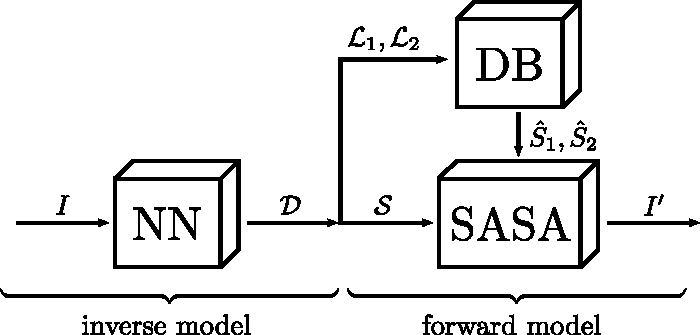
\includegraphics[width=.63\linewidth]{al_combined}
    \caption{A part of the algorithm described in section \ref{sec:algorithm} can be understood as a tandem model 
    $I \rightarrow \mc D \rightarrow I'$.
    This combined model receives a target spectrum and outputs its best reproduction of that spectrum $I'$. The notation is the same as in figure \ref{fig:al:algo}.}
    \label{fig:al:combined}
\end{figure}


This combined model can easily be implemented as all the necessary modules are already there but it can not be trained. To understand why we need to go back to the concept of {\hyperref[eq:bg:back_prop]{Backpropagation}}.
During training the gradient of the cost function needs to propagate backwards through the network. To capture this mathematically we will identify the forward model in figure \ref{fig:al:combined} as the last layer $L$ in a combined network. Equation \eqref{eq:bg:back_prop} tells us we need to calculate:

\begin{equation}
    \delta^L_j = \pdv{C}{a^L_j} \ \pdv{a^L_j}{z^L_j}
\end{equation}

The first part $\partial C / \partial{a^L_j}$ is simple and only depends on the cost function. For example for \\
$C_\s{mse} = \sum_j \qty(a_j^L - y_j)^2$
the derivative is 
$\partial{C} / \partial{a^L_j} = 2 \qty(a_j^L - y_j)$
but the second part 
$\partial{a^L_j} / \partial{z^L_j}$
the output of the last layer derived by the input to the last layer is not easily accessible. Maybe not accessible at all if we consider the calls to the database and interpolation that happen during this step. The only way to train this combined tandem model is by replacing the forward model with something where we can access the gradient.


\paragraph{Network Architecture}~\\
The network architecture we used for the inverse problem contained pooling layers to gradually reduce the many parameters of a spectrum $I$ to a few design parameters $\mc D$. Here we have to go the opposite way and upsample $\mc D$ to $I$. For this we will use upsampling layers which double the size of their input, e.g. $(1,3) \rightarrow (1,1,3,3)$. The convolution is then applied to this upsampled output to "fill in the details" \cite{fill_in_details}. This combination of upsampling and convolution is called \textit{transposed convolution} in literature \cite{TransposedConv}. The full Network architecture is shown in figure \ref{fig:in:NN} and contains two more new layers. Batch Normalization (BN) and a running average filter (Avg).
\\

\indent
Batch Normalization was introduced by Ioffe and Szegedy in 2015 \cite{Ioffe2015}. This layer calculates the mean $\mu_\mc B$ and variance $\sigma_\mc B$ over every \hyperref[hyp:minibatch]{mini-batch} $\mc B$. Then it normalizes the output of the previous layer $\vb x$ to 
\begin{equation}
    \bar x_i = \frac{x_i - \mu_\mc B}{\sigma_\mc B}
    \qq{and rescales it to}
    y_i = \gamma \bar x_i + \beta \,,
\end{equation}

where $\gamma$ and $\beta$ are trainable parameters. This way the output of the previous layer has a mean of zero and a variance of one which has advantages for the networks stability and training speed \cite{Ioffe2015}.
(Batch Normalization was later also added to the inverse model.)
Additionally, the running average filters were added because the output oscillated too much on small wavelength differences.
This way the fact, that transmission spectra do not change too much on a per wavelength scale, is directly contained in the network architecture. 
\\

\begin{figure}[H]
    \centering
    \includegraphics[width=\linewidth]{in_NN_architecture}
    \caption{Network architecture of the forward model. First the discrete and continuous inputs are combined and connected to a Dense layer with 
    $(20 \cdot 128)$
    neurons. The number 20 will later become 160 discretized wavelength after the three upscale operations are applied. As discussed in section \ref{sec:NN_bg} convolutional layers operate on stacked feature maps. This is why the $20 \cdot 128$ flat neurons need to be reshaped into a $20 \times 128$ array. Next there are three transposed convolutional layers $CNU$. Each consisting on a basic convolution $C$, a Batch Normalization $N$ and an upscale layer $U$. The convolution is characterized by the parameters (\textit{number of kernels, kernel size}). The final convolution $C^4$ reduces the number stacked feature maps to 2. One each for the $x$ and $y$ polarization. Finally, two running average filters (Avg) are applied to smooth the output. All the internal activations $\sigma_\s{r}$ are ReLu's and the final activations $\sigma_{l}$ is a linear function.
    Layers which contain trainable parameters are marked red.
    }
    \label{fig:in:NN}
\end{figure}



\newpage
\paragraph{Network Training}~\\
The forward model is trained like the inverse model just the inputs and outputs are exchanged. That is, the training data $(X,\, Y)$ now consists of tuples 
$(\mc D,\, I)$ instead of $(I,\, \mc D)$.
This allows us to use the same underlying data of pre simulated stacks, we already have, to also train the forward model. 
The mean absolute error (mae) per spectrum drops to 0.04 over 20 epochs as shown in figure \ref{fig:in:forward_training}. $I$ consists of 160 discretized wavelengths for two polarizations. This means the transmission at every wavelength is on average $4/320 = 1/30$ percent points off. However, the forward model is not perfect. As can be seen in figure \ref{fig:in:avg_plot} it generates small troughs and peaks where there are none in the original spectrum.
\\

\indent
Now we can combine the inverse model $\mc D \rightarrow I$ and the forward model $I \rightarrow \mc D$ into a combined model $I \rightarrow \mc D \rightarrow I'$ and directly use the loss function $C_\s{mse}(I,\, I')$.
However, even trying different regularization techniques, this model could not be trained successfully as seen in figure \ref{fig:ap:combined_training}.  


\begin{figure}[H]
    \floatbox[{
    \capbeside
    \thisfloatsetup{capbesideposition={right,top}}}]{figure}[\FBwidth]
    {\caption{
        Training of the forward model. The Network performance is evaluated based on the mean absolute error (mae). If $I$ is the real spectrum and $I'$ is the networks output then 
        $C_\s{mae} = \sum_i \qty|I_i - I'_i|$.
    }
    \label{fig:in:forward_training}}
    {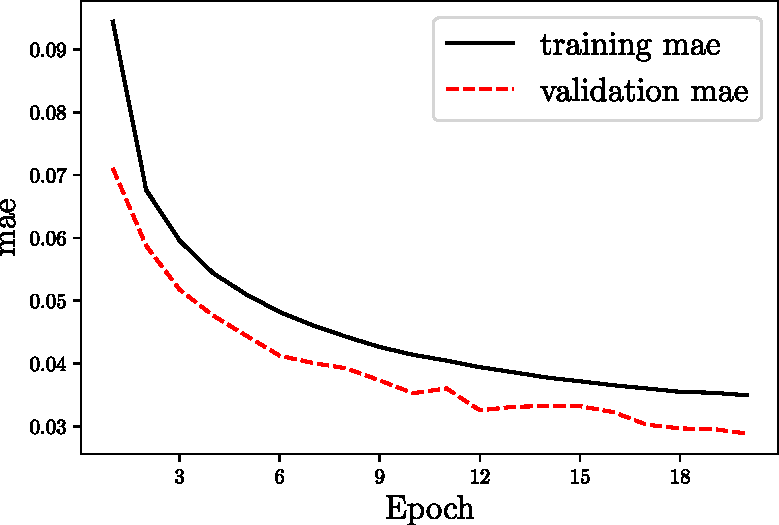
\includegraphics[width=0.6\textwidth]{in_forward_training}}
\end{figure}

\begin{figure}[H]
    \floatbox[{
    \capbeside
    \thisfloatsetup{capbesideposition={right,top}}}]{figure}[\FBwidth]
    {\caption{
        Training of the combined model. Validation loss oscillates wildly.
    }
    \label{fig:ap:combined_training}}
    {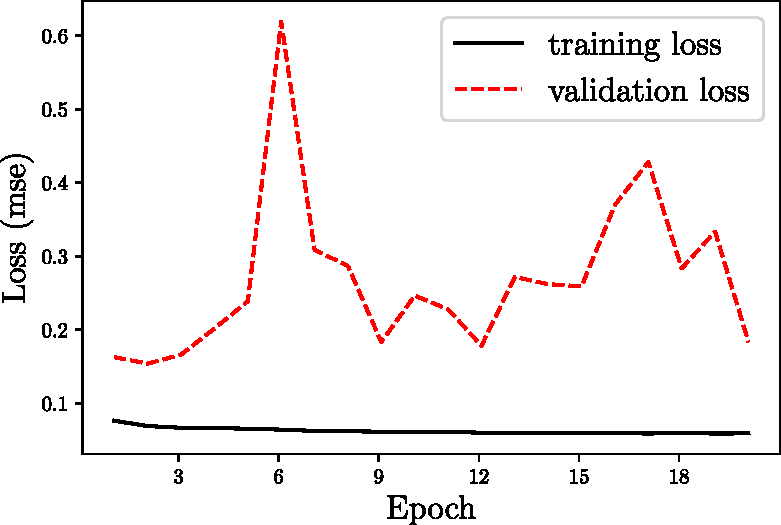
\includegraphics[width=0.6\textwidth]{ap_combo}}
\end{figure}

\newpage

\section{Example Fits}\label{sec:apdx_B}
Some example fits. All figures show the transmission over the wave length in $\mu$m from $0.4\, \mu \s m$ to $1.2\, \mu \s m$.
All parameters are given in nm except for the angle in degree and the spacer hight in $\mu$m.
\begin{figure}[H]
\centering
\begin{subfigure}{.5\textwidth}
    \centering
    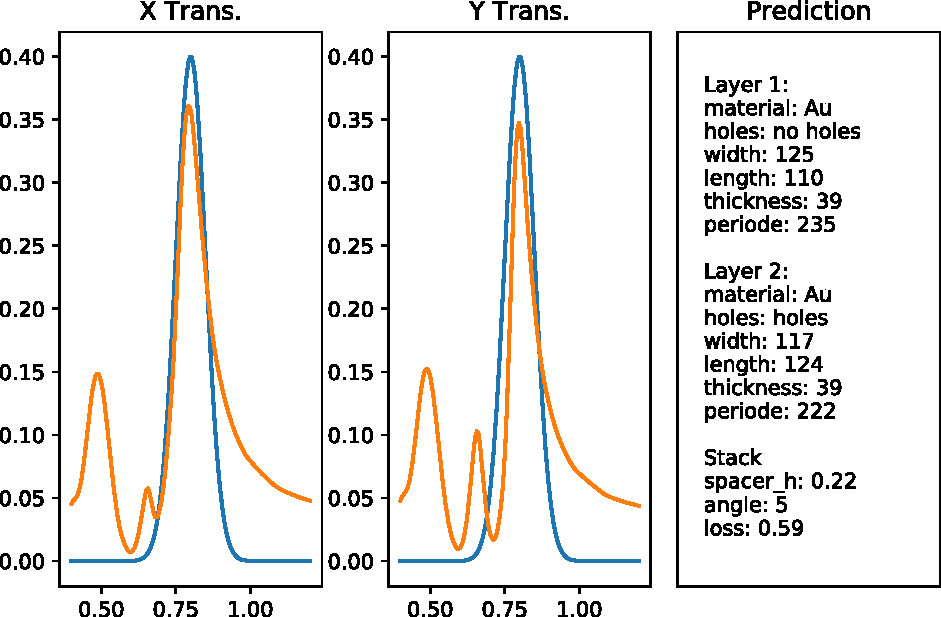
\includegraphics[width=\linewidth]{ap_peak2.pdf}
    \caption{Gauß Peak}
    \label{gauspeak}
\end{subfigure}%
\begin{subfigure}{.5\textwidth}
    \centering
    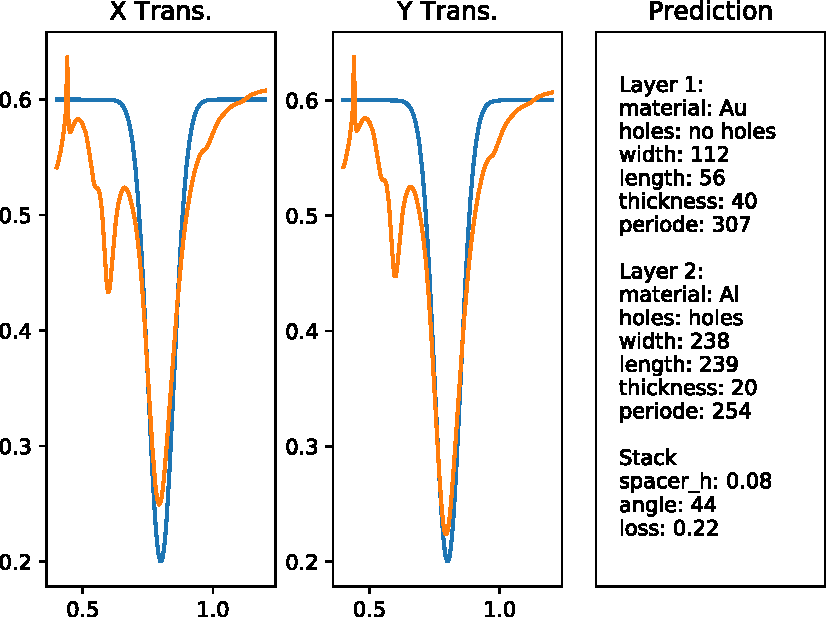
\includegraphics[width=.9\linewidth]{ap_dip2.pdf}
    \caption{Gauß Dip}
    \label{gausdip}
\end{subfigure}
\caption{}
\label{}
\end{figure}


\begin{figure}[H]
\centering
\begin{subfigure}{.5\textwidth}
    \centering
    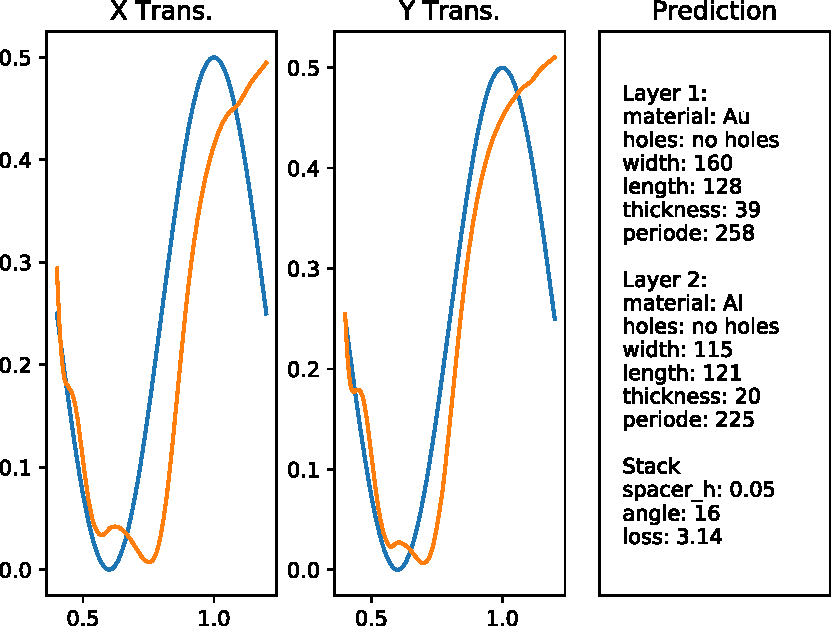
\includegraphics[width=\linewidth]{ap_sine2}
    \caption{Sine}
    \label{}
\end{subfigure}%
\begin{subfigure}{.5\textwidth}
    \centering
    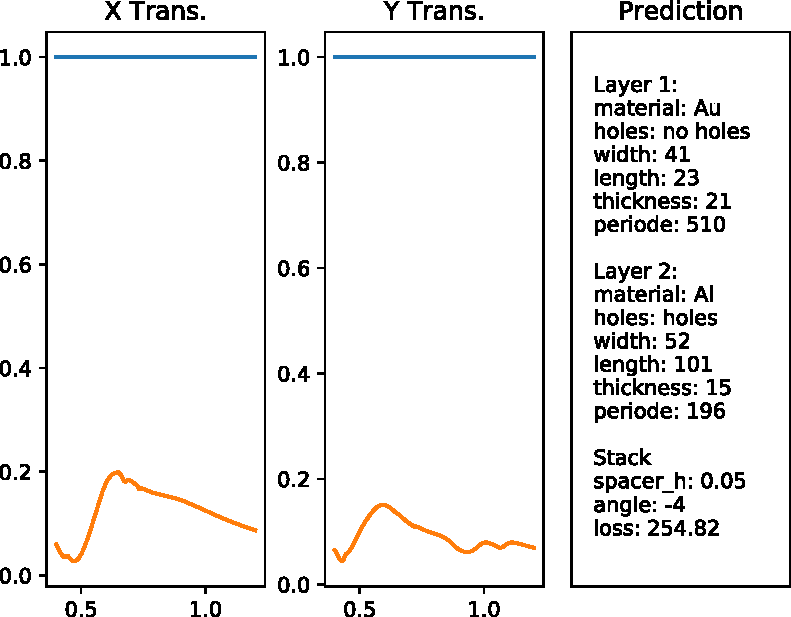
\includegraphics[width=.95\linewidth]{ap_one2}
    \caption{Failed fit on an all one transmission spectrum.}
    \label{one}
\end{subfigure}
\caption{}
\label{}
\end{figure}

\begin{figure}[H]
    \floatbox[{
    \capbeside
    \thisfloatsetup{capbesideposition={right,top}}}]{figure}[\FBwidth]
    {\caption{
        Here, the two sets of layer parameters from figure \ref{gausdip} were directly simulated via FMM and then the transmission spectrum was calculated via SASA. The agreement of this transmission spectrum and figure \ref{gausdip} indecates that the interpoation of $S$-matrices is working correctly.
    }
    \label{fig:in:avg_plot}}
    {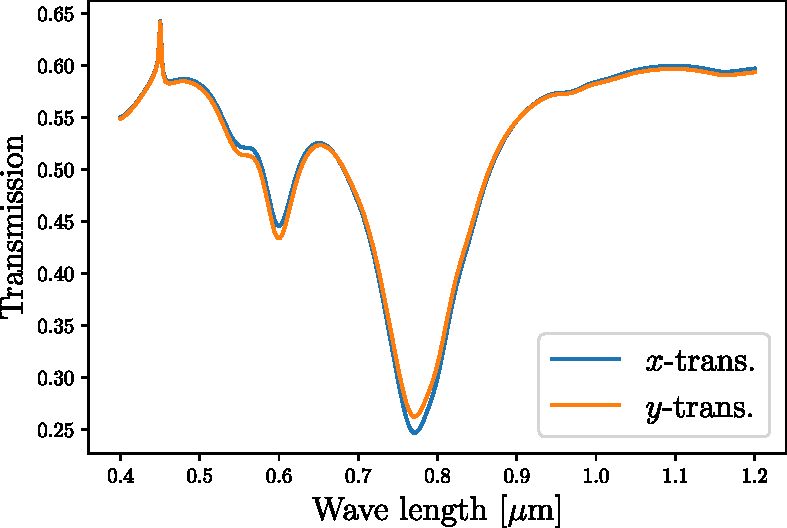
\includegraphics[width=0.5\textwidth]{ap_simul}}
\end{figure}